\documentclass{article}
\usepackage{amssymb}
\usepackage{amsmath}
\usepackage{centernot}
\usepackage{graphicx}
\begin{document}
\title{\vspace{-60px}M351K\: Homework 1}
\author{Joshua Dong}
\date{\today}
\maketitle

\section*{1: Two Dice}
\subsection*{a)}
The sample space for the two dice rolls is $\{1, ..., 6\} \times \{1, ..., 6\}$,
or explicitly: $
\{(1,1),(1,2),(1,3),(1,4),(1,5),(1,6),
\\(2,1),(2,2),(2,3),(2,4),(2,5),(2,6),
\\(3,1),(3,2),(3,3),(3,4),(3,5),(3,6),
\\(4,1),(4,2),(4,3),(4,4),(4,5),(4,6),
\\(5,1),(5,2),(5,3),(5,4),(5,5),(5,6),
\\(6,1),(6,2),(6,3),(6,4),(6,5),(6,6)\}
$

\subsection*{b)}
If $A$ is the set of events where the number of dots in first toss is not less
than number of dots in second toss, then
\\
$A = \{(1,1),(2,1),(2,2),(3,1),(3,2),(3,3),(4,1),(4,2),(4,3),(4,4),
\\(5,1),(5,2),(5,3),(5,4),(5,5),(6,1),(6,2),(6,3),(6,4),(6,5),
(6,6)\}
$.

\subsection*{c)}
If $B$ is the event where the number of dots in first toss is 6, then
\\
$B = \{(6,1),(6,2),(6,3),(6,4),(6,5),(6,6)\}$.

\subsection*{d)}
$A \cap B^c = \{(1,1),(2,1),(2,2),(3,1),(3,2),(3,3),(4,1),(4,2),(4,3),
\\(4,4),(5,1),(5,2),(5,3),(5,4),(5,5)\}$.
\\This is the event that the first die roll has more dots
facing up than the second die roll but the first roll was not 6.

\subsection*{e)}
Let $C$ be the event that the mangitude of the difference of dots between
the two die rolls is two.
\\Then $A \cap C = \{(3,1),(4,2),(5,3),(6,4)\}$.

\section*{2: Names in a Hat}
\subsection*{a)}
The sample space is the permutation of their names:
\\ $\{(Al,Bob,Chris),(Al,Chris,Bob),(Bob,Al,Chris),
\\ (Bob,Chris,Al),(Chris,Al,Bob),(Chris,Bob,Al)\}$.

\subsection*{b)}
$A = \{(Al,Bob,Chris),(Al,Chris,Bob)\}$.
\\ $B = \{(Al,Bob,Chris),(Chris,Bob,Al)\}$.
\\ $C = \{(Al,Bob,Chris),(Bob,Al,Chris)\}$.

\subsection*{c)}
$\{(Bob,Chris,Al),(Chris,Al,Bob)\}$

\subsection*{d)}
$\{(Al, Bob, Chris)\}$

\subsection*{e)}
$A \cup B \cup C =
\\\{(Al,Bob,Chris),(Al,Chris,Bob),(Chris,Bob,Al),(Bob,Al,Chris)\}$.

\section*{3: Set Algebra}
We want to show that
\\ $A \cup B \cup C = A + B + C - (A \cap B) - (B \cap C) -
(C \cap A) + (A \cap B \cap C)$.
\\
\\ $A \cup B \cup C =
\\ (A \cup B) \cup C = 
\\ (A + B - (A \cap B)) \cup C = 
\\ (A + B - (A \cap B)) + (C) - ((A + B - (A \cap B)) \cap C) = 
\\ A + B + C - (A \cap B) - ((A \cap C) + (B \cap C) - ((A \cap B) \cap C)) = 
\\ A + B + C - (A \cap B) - (A \cap C) - (B \cap C) + (A \cap B \cap C).$
\\ Which is what we sought to show.

\newpage

\section*{4: Venn Diagrams}
\begin{figure}[h]
  \centering
  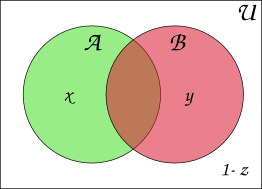
\includegraphics[width=0.5\textwidth]{Venn.png}
  \vspace{-16px}
\end{figure}
$
\\ P[A \cap B] = x + y - z.
\\ P[A^c \cap B^c] = 1 - P[A \cup B] = z.
\\ P[A^c \cup B^c] = 1 - P[A \cap B] = 1 - x - y + z.
\\ P[A \cap B^c] = P[A] - P[A \cap B] = x - (x + y - z) = z - y.
\\ P[A^c \cup B] = 1 - P[A \cap B^c] = 1 - z + y.
$


\section*{5: Counting}
\subsection*{a)}
There are $100 \cdot 100 \cdot 100$ or $1,000,000$ unique lock positions.

\subsection*{b)}
There are $6 \cdot 6 \cdot 2 \cdot 2 \cdot 52$ or $7488$ unique outcomes.

\section*{6: Pizza}
With repeats, there are $15 \cdot 15 \cdot 15 \cdot 15 \cdot$ or $50625$ unique
pizza types. With no repeats, there are $15 \choose 4$ or $1365$ unique pizza
types.

\section*{7: Passwords}
There are $14 + 10 + 26 + 26$ or $76$ choices for each character. Passwords
may be 8, 9, or 10 characters long. Then there are $76^8 + 76^9 + 76^{10}$ or
$6514592610973974528 \approx 5 \cdot 2^{60}$ unique passwords. Brute forcing at
1 password per microsecond sequentially would take just under 206500 years, at
worst. Note however, that with proper brute forcing technique and modern
machines, this password is not necessarily secure.

\end{document}
